\documentclass{beamer}

\usepackage[utf8]{inputenc}
\usepackage{subfig}
\usepackage{ngerman}
\usetheme{Singapore}

% Captions
\usepackage{caption}
\captionsetup[figure]{labelformat=empty}

% Bibliography
\usepackage[citestyle=numeric,style=numeric,backend=biber]{biblatex}
\addbibresource{bibliography.bib}

\title{Prozedurale Generierung\\ von Wirbeltierskeletten}
\author{Nina Zimbel}
\institute{KIT - Institut für Visualisierung und Datenanalyse}
\date{\today}

\begin{document}

\begin{frame}
 \maketitle
\end{frame}

% \begin{frame}[focus]
%  \centering
%  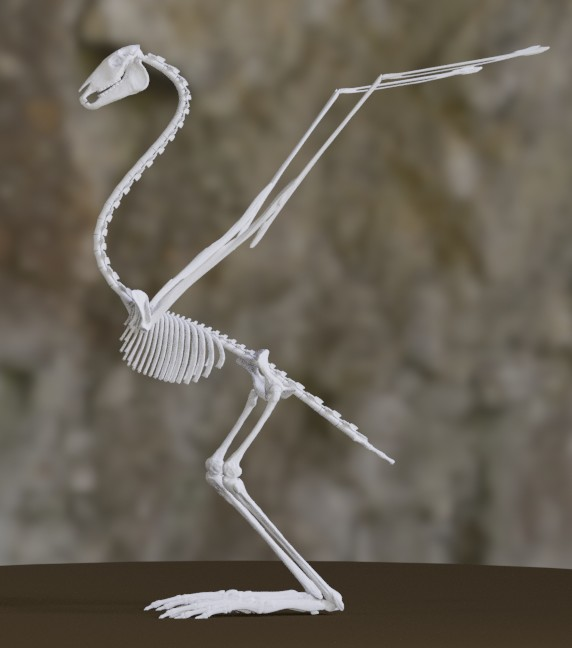
\includegraphics[height=\textheight]{../../java_skeleton_generation/example_skeletons/bird.jpg}
% \end{frame}

\section{Einleitung}
\begin{frame}
 \begin{figure}
  \centering
  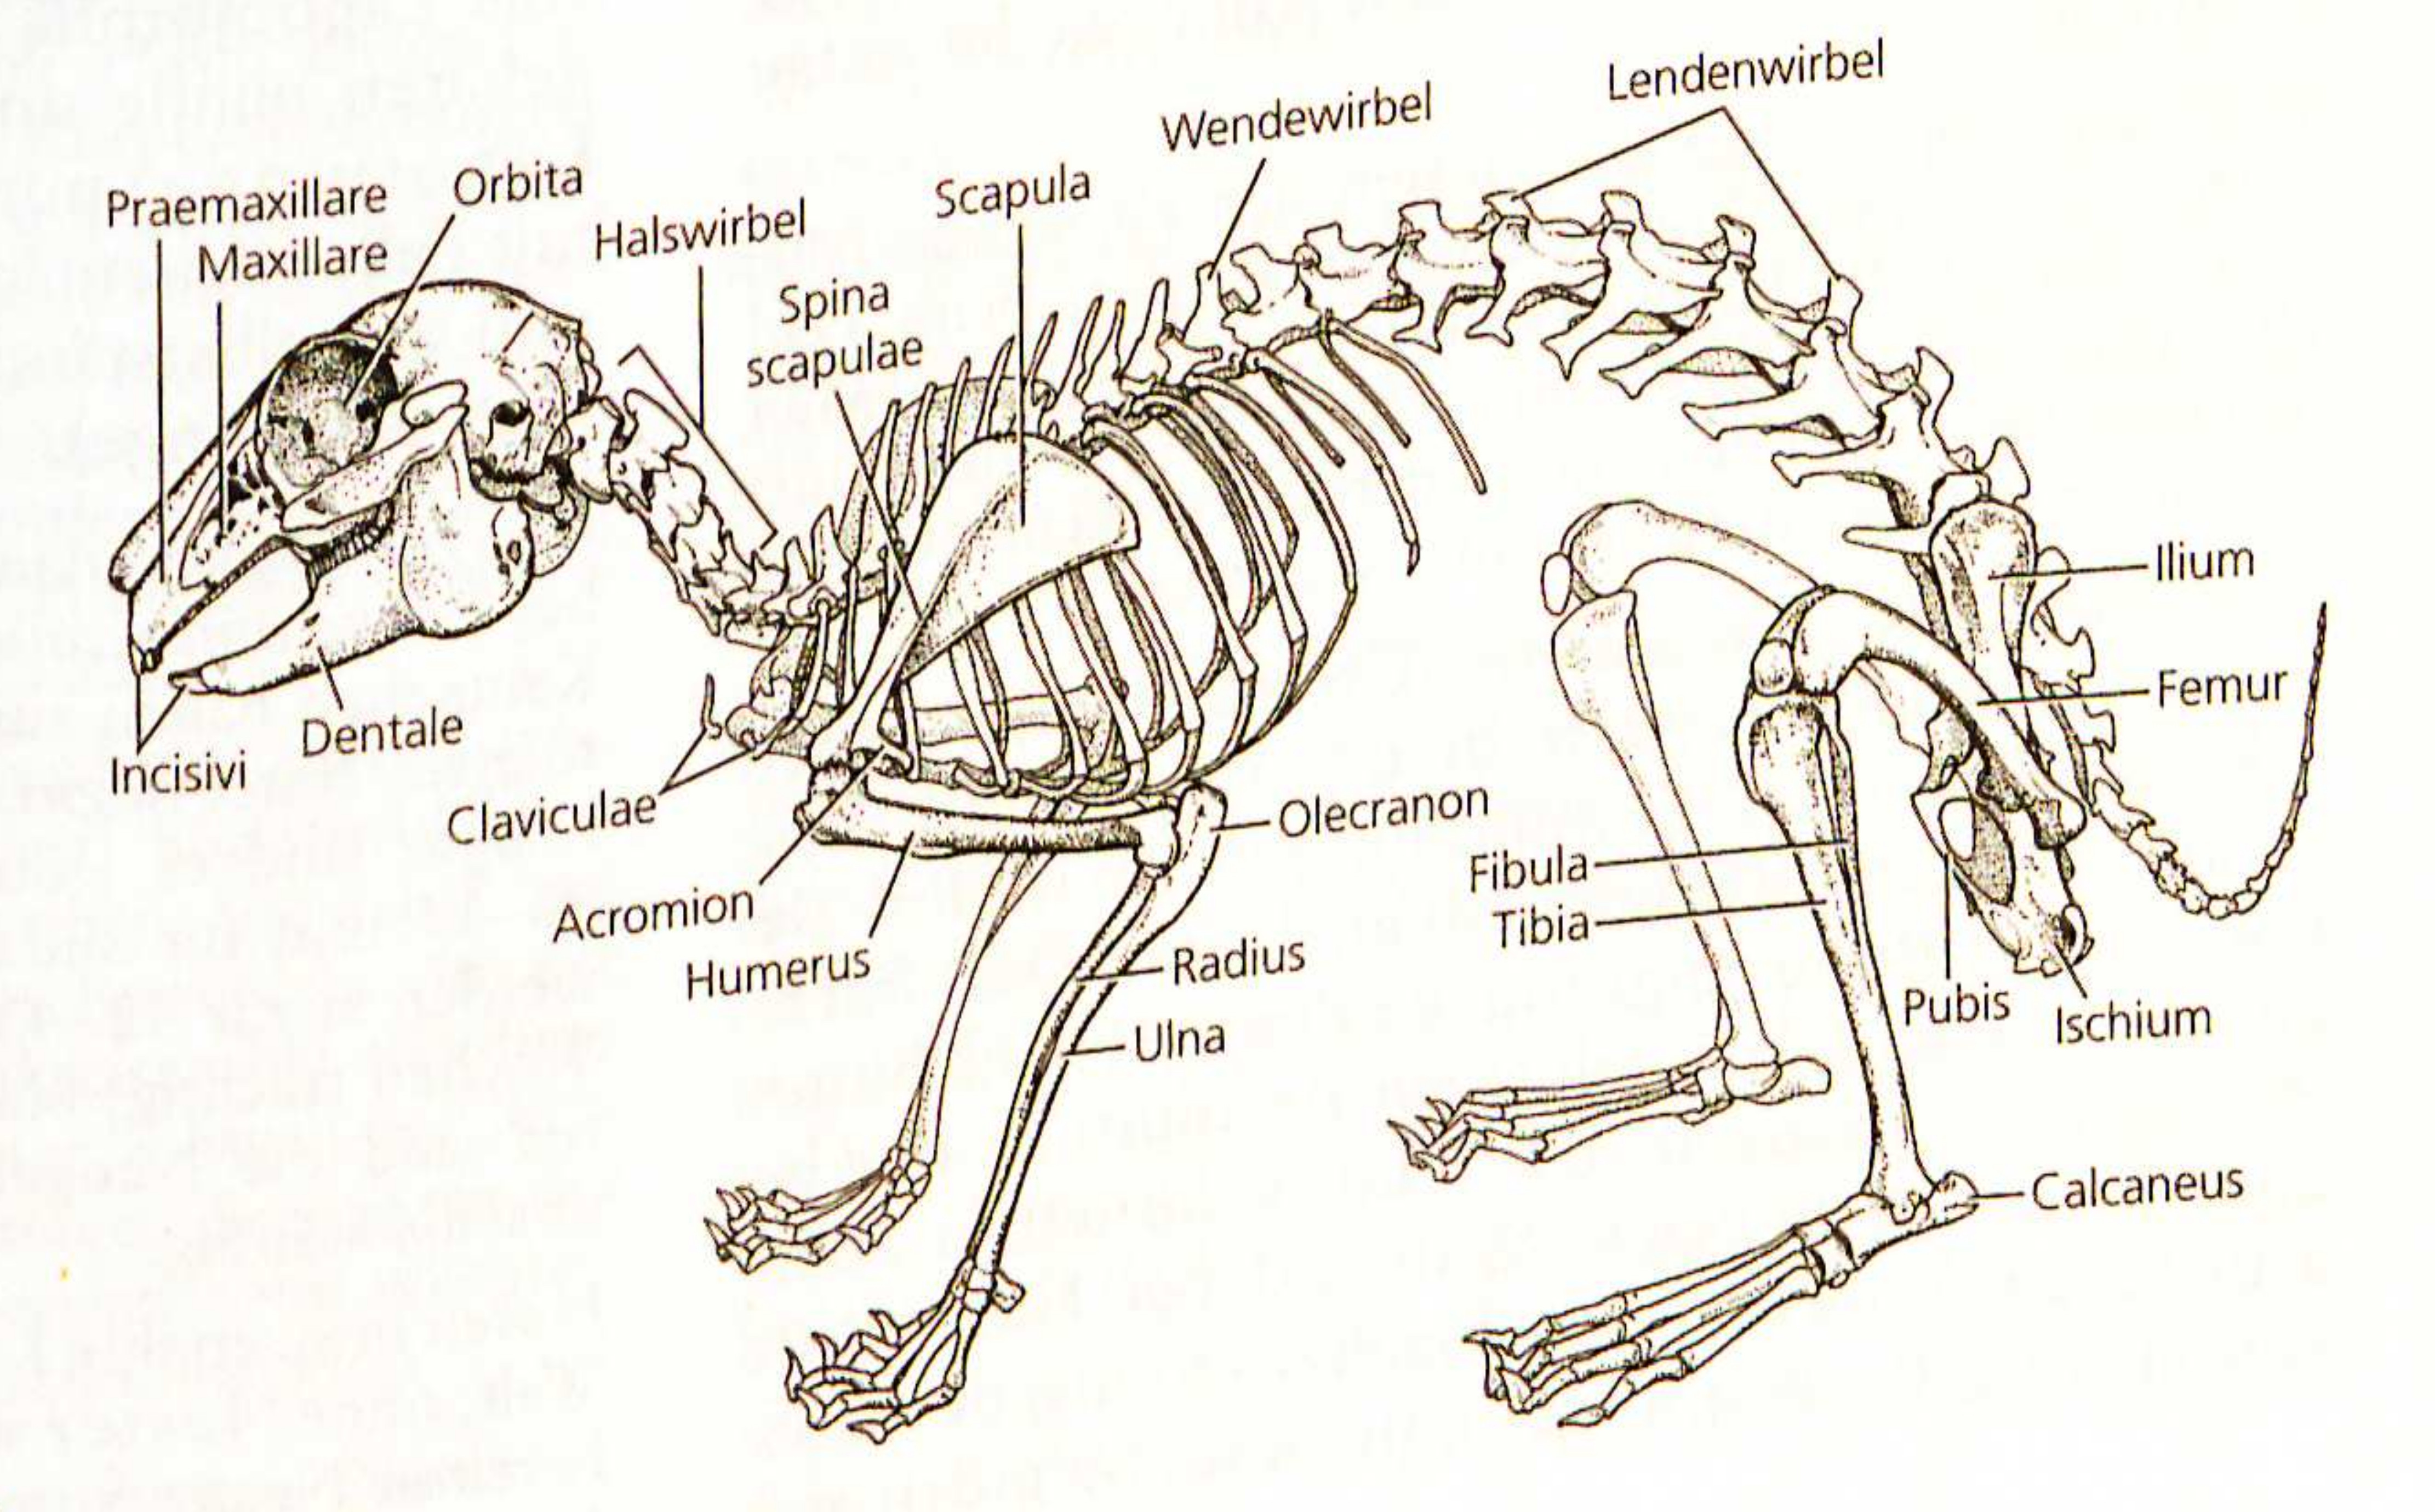
\includegraphics[width=\textwidth]{graphics/kaninchen.jpg}
  \caption{Skelett eines Kaninchens \cite{Spezielle_Zoologie}}
 \end{figure}
\end{frame}

\begin{frame}
 \begin{figure}
  \centering
  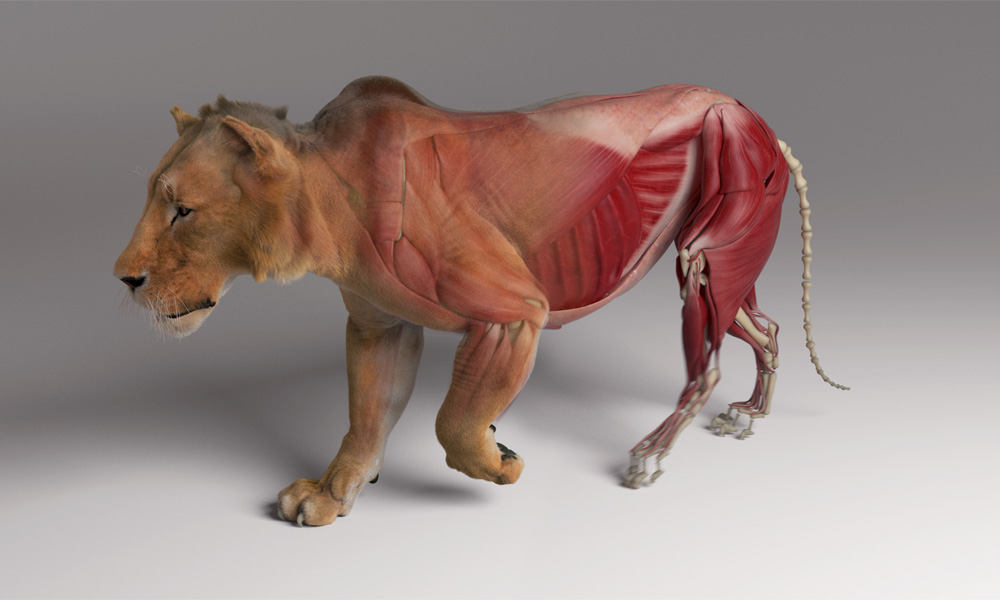
\includegraphics[width=\textwidth]{graphics/ziva-post2.jpg}
  \caption{Maya Plugin Ziva, wirklichkeitsgetreues Modell eines Löwen \cite{Ziva_Lion}}
 \end{figure}
\end{frame}

\begin{frame}
 \begin{figure}
  \centering
  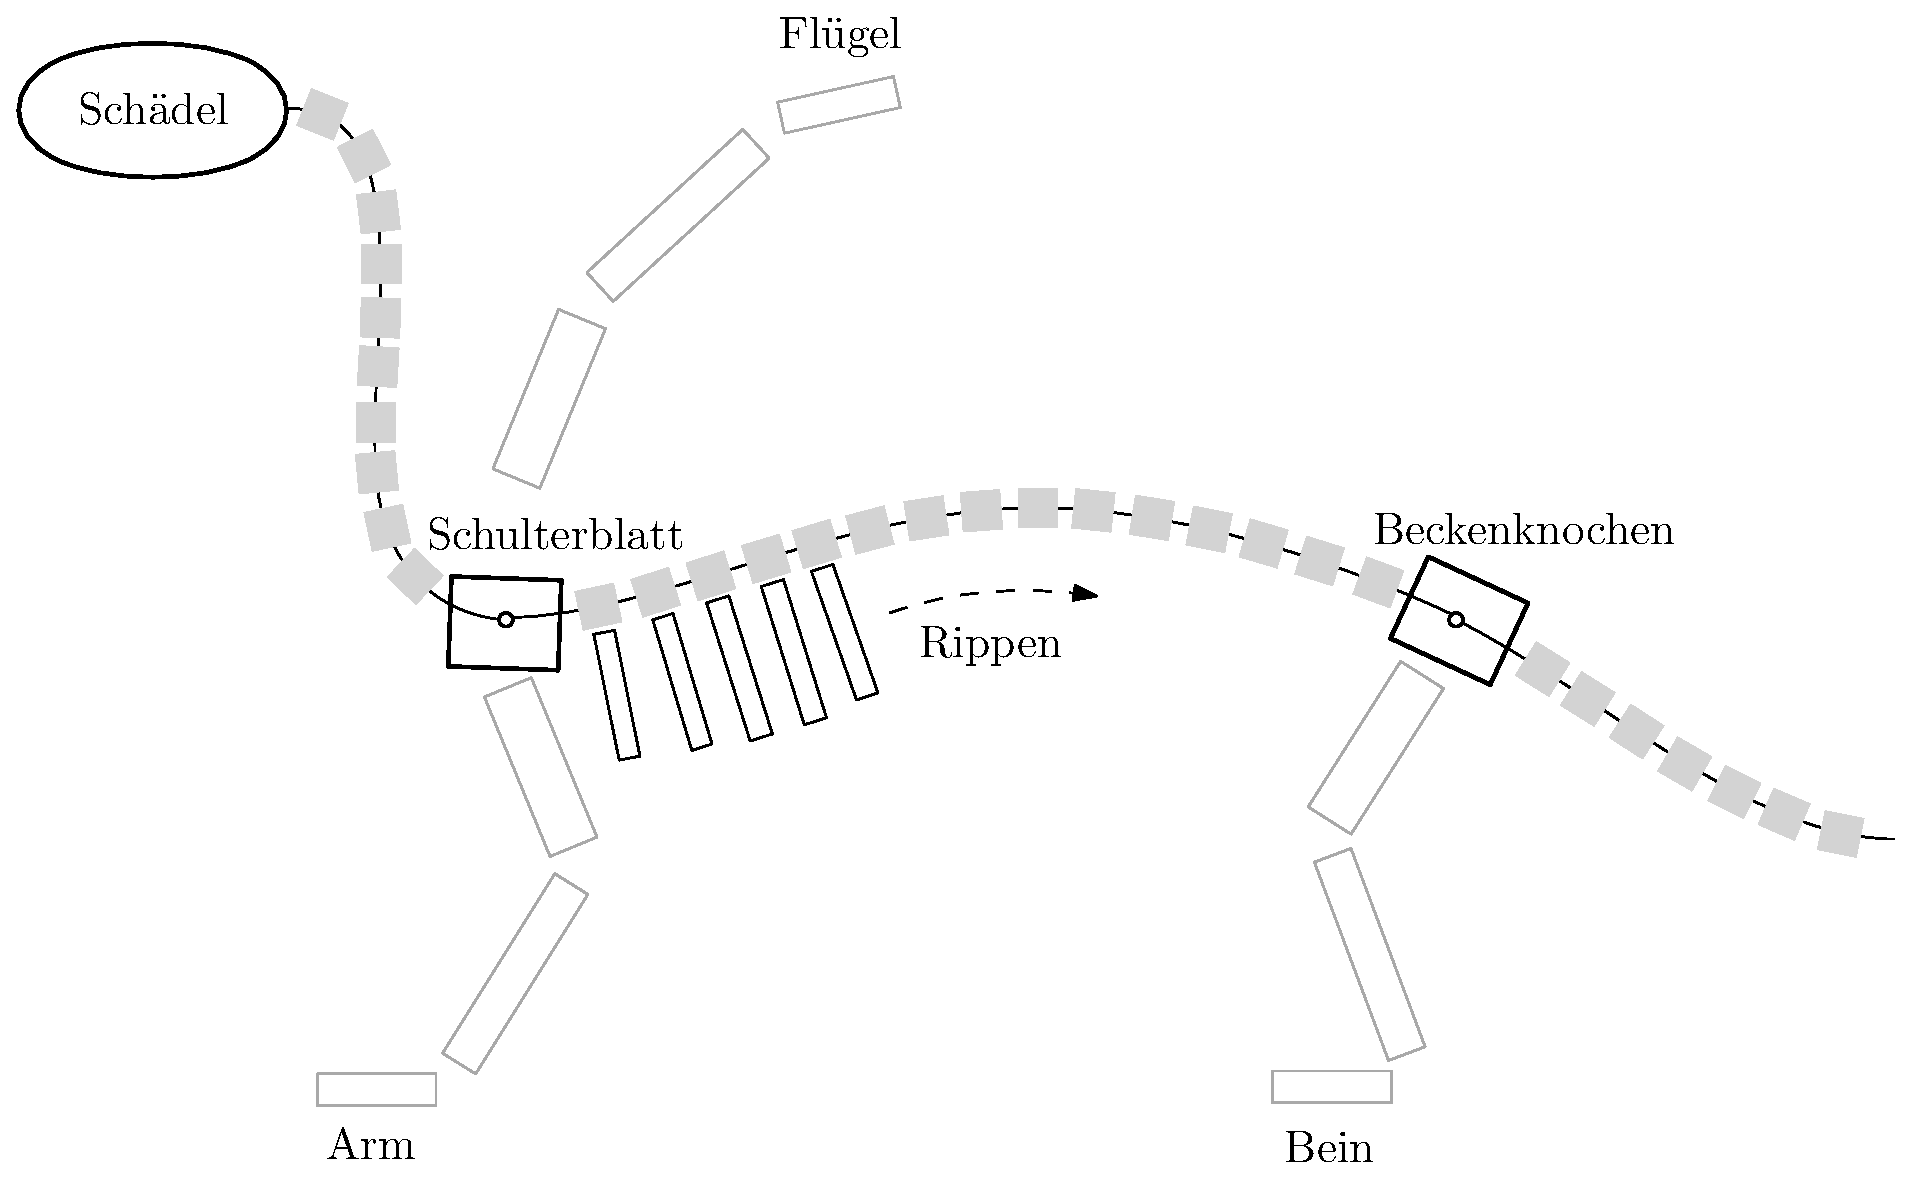
\includegraphics[width=\textwidth]{../graphics/skeletonPlan}
  \caption{Abstrahierter Grundbauplan eines Wirbeltierskeletts}
 \end{figure}
\end{frame}


\section{Principal Component Analysis}
\begin{frame}{Warum Principal Component Analysis (PCA)?}
 \only<1>{
  \begin{figure}
   \centering
   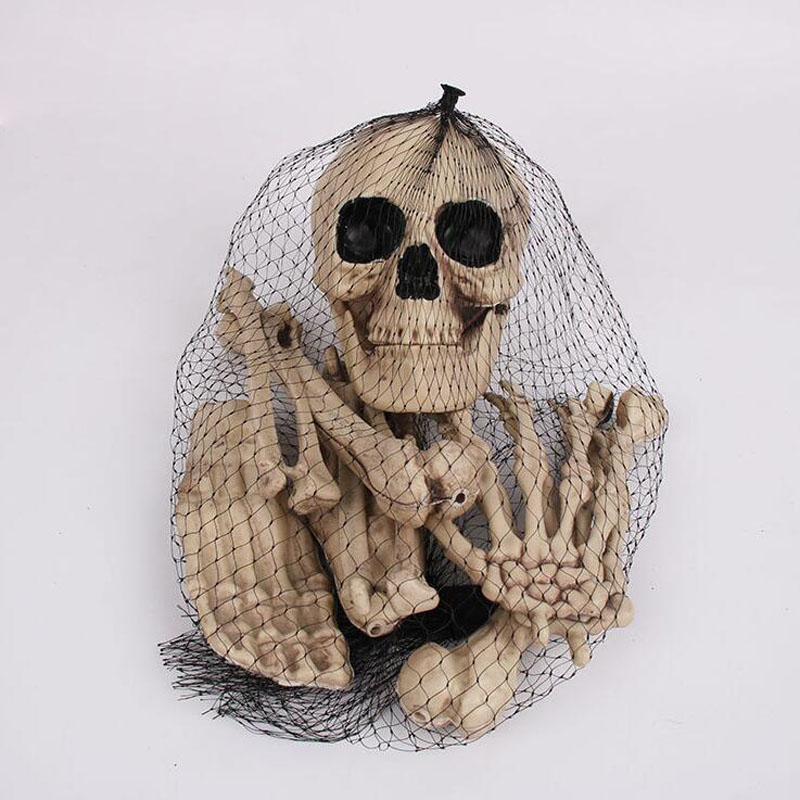
\includegraphics[height=0.7\textheight]{graphics/skeleton_set.jpg}
   \caption{\cite{skeleton_set}}
  \end{figure}
 }
 \only<2->{
  \begin{figure}
   \centering
   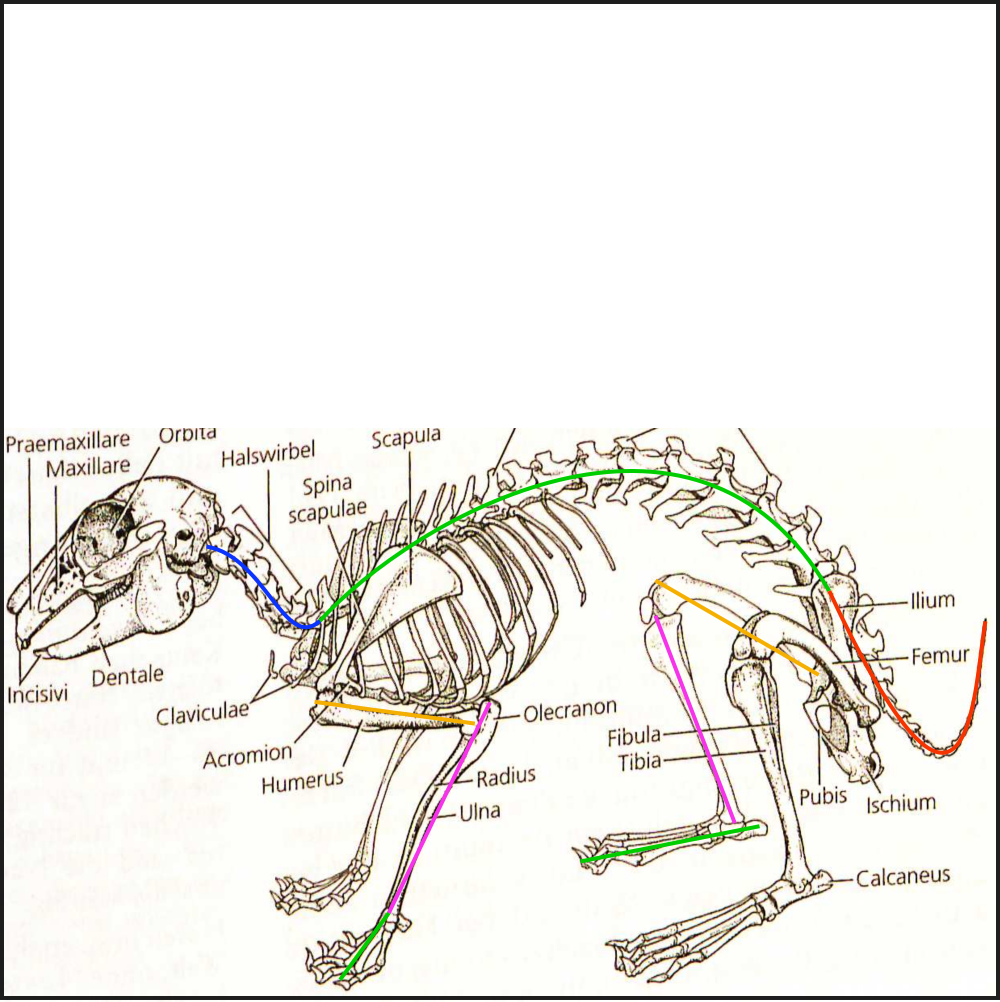
\includegraphics[height=0.7\textheight]{../../PCA/Skelettbilder/Kaninchen_farbig.png}
   \caption{Annotiertes Skelett eines Kaninchens, zusätzlich erhobene Merkmale: Anzahl \emph{Flügel}, Anzahl \emph{Beine} mit Bodenkontakt, \emph{Gewicht}}
  \end{figure}
 }
\end{frame}

\begin{frame}{PCA}
 Wie funktioniert PCA?
\end{frame}



\begin{frame}
 \printbibliography[heading=bibintoc]
\end{frame}


\end{document}
